%\subsection{Patching In The Toolchain}
{\bf Patching In The Toolchain.}
\label{ssec:patchingvlinking}
Hot patching should not be thought of as a bizarre operation, done
crudely and infrequently, something akin to reverse engineering. We
argue that it is one of the fundamental transformations in the life
cycle of any program, along with compilation, linking, dynamic
linking, and (in unfortunate cases) dumping core. We note that each of
these fundamental operations has its own type of ELF object devoted to
it (relocatable objects, executables, dynamic libraries, core dumps
respectively) and a corresponding tool in the toolchain for effecting
each transformation or working with its output. \emph{We contend that
patching is very much like linking or dynamic linking}. Like those
operations, it combines (or replaces) parts of programs and must
generate, modify, and apply relocation information. The section types
defined for the ELF format contain nearly all of the information
necessary to describe a patch. Once we take the position that patching
is like linking, it follows that a patch needs to store the same type
of symbol and relocation information as does any relocatable ELF
object.

What the base ELF specification lacks is a way to describe
types. Symbol information gives us only a location and a length, but
there is no way to describe the internal layout of a piece of
data. The DWARF format, already heavily used with ELF for debugging
and exception-handling purposes, provides exactly what is needed here
as it provides a means to recursively describe types and variables, as
well as a set of instructions originally designed for restoring
register states and examining the call stack but rich in possible
applications. 

Through the use of formats already employed in the binary tool chain, we
hope to promote easy examination of patches, interoperability, and to
show that patching fits comfortably into the rest of the
toolchain. We therefore propose that the standard software life cycle
now be as shown in Figure \ref{fig:lifecycle}. Before hot
patching, only the Development and Runtime stages of the figure were
generally accepted.

\begin{figure}[ht]
\begin{center}
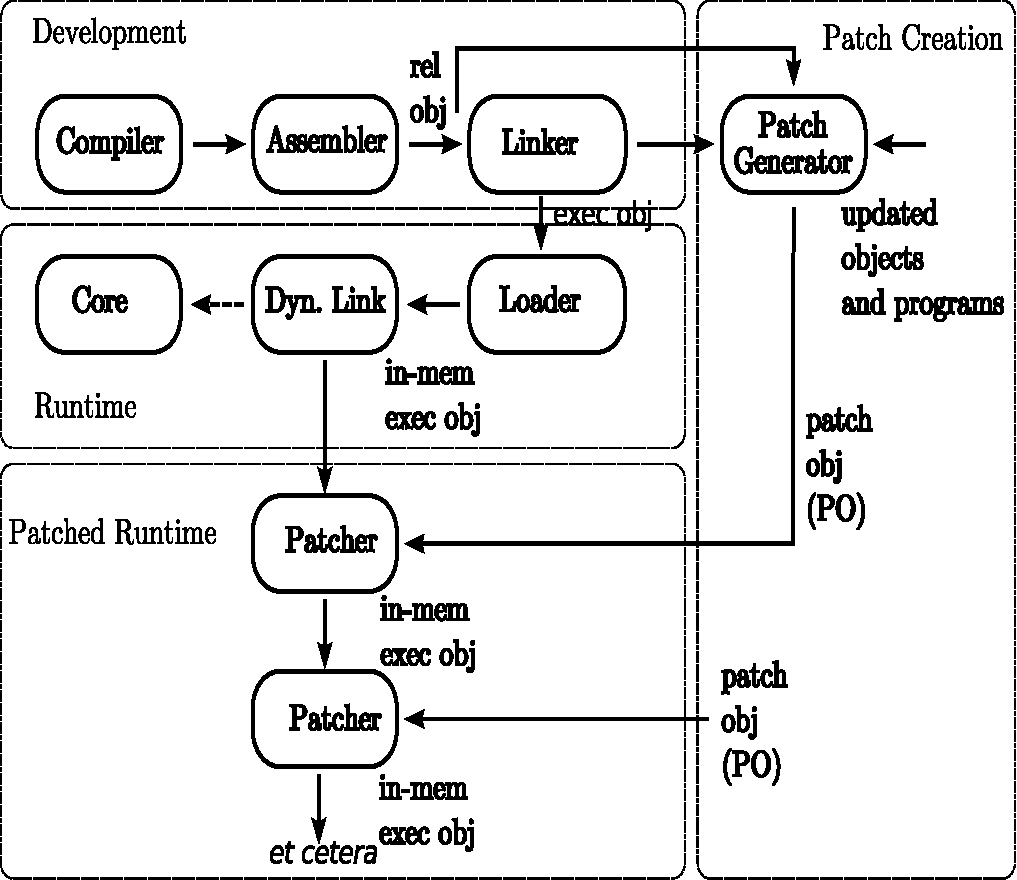
\includegraphics[scale=0.5]{software_lifecycle.pdf}
\end{center}
\caption{{\small Revised software life cycle. Before hot patching, only
    the Development and Runtime portions existed}}
\label{fig:lifecycle}
\end{figure}

% LocalWords:  toolchain
